\section{Primal-Dual IPM}
Previously, we discussed Barrier Methods and the so-called short-step method for solving constrained LPs, and proved that convergence is guaranteed (albeit slow). Herein, we study a primal-dual interior-point method (the so-called "long-step"  path following algorithm), which similarly seeks to approximate points on the central path. Unlike the short-step method, the long-step method considers iterates of Primal-Dual variables and seeks a more aggressive step size so long as it lies within a neighborhood of the central path.



\subsection{Deriving the dual problem}

Let $x \in \R^n$ be the decision variable, and $A \in \R^{m \times n},b \in \R^m$ and $c \in \R^n$
\begin{eqnarray*}
\min c^\top x \quad \text{s.t.}\quad Ax = b, x \ge 0 
\end{eqnarray*}
Here, $\ge$ is pointwise.

Observe that we can always write the constraint as 
\begin{eqnarray*}
&& \min_{x \ge 0 } c^\top x + \max_{z} z^{\top}(b-Ax) \\
&=& \min_{x \ge 0} \max_{z} c^\top x + \max_{z} z^{\top}(b-Ax) \\
&\ge& \max_{z} z^{\top}b - \min_{x \ge 0} (c - A^{\top}z)^{\top}x\\
&=& \max_{z} z^{\top}b  - \infty \cdot \Ind(A^{\top}z > c)\\
\end{eqnarray*}
Hence, the dual problem is as follows
\begin{eqnarray*}
\max b^\top z \quad \text{s.t.}\quad A^{\top} z \le c
\end{eqnarray*}
This is equivalent to 
\begin{eqnarray*}
\max b^\top z \quad \text{s.t.}\quad A^{\top} z + s = c, \quad s \ge 0
\end{eqnarray*}
where we introduce the slack variable $s \in \R^n$. If $(x,z,s)$ are only \emph{feasible}, then 
\begin{eqnarray*}
Ax = b \quad A^{\top} z + s = c \quad x,s \ge 0
\end{eqnarray*}
Moreover, we can compute that for feasible $(x,z,s)$,
\begin{eqnarray*}
0 \le \langle x, s \rangle = x^{\top}(c - A^{\top}z) = \langle x, c \rangle - \langle Ax, z \rangle = \langle x, c \rangle - \langle b,z \rangle~.
\end{eqnarray*}
This is a proof of weak duality, namely that for any feasible $x$ and $z$,
\begin{eqnarray*}
\langle x, c \rangle  \ge \langle b,z \rangle
\end{eqnarray*}
and therefore
\begin{eqnarray*}
\langle x^*, c \rangle  \ge \langle b,z^* \rangle
\end{eqnarray*}
Moreover, if there exists an feasible $(x^*,z^*,s^*)$, with $\langle x^*, s^* \rangle = 0$ then we have 
\begin{eqnarray*}
\langle x^*, c \rangle = \langle b^*,z \rangle~
\end{eqnarray*}
which is strong duality. 

Duality is also useful to bound the suboptimality gap, since in fact if $(x,z,s)$ is feasible, then
\begin{eqnarray*}
\langle x, s \rangle = \langle x, c \rangle - \langle b,z \rangle \ge \langle x,c \rangle - \langle x^*, c \rangle = \langle x - x^* , c \rangle
\end{eqnarray*}

\subsection{Primal-dual iterates along the central path}
The above suggests the following approach. Consider iterates $(x_k,z_k,s_k)$, and define
\begin{eqnarray*}
\mu_k := \frac{1}{n}\cdot \langle x_k, s_k \rangle = \frac{\langle x_k, c \rangle - \langle b,z_k \rangle}{n} \ge \frac{\langle x_k-x^* , c \rangle}{n}
\end{eqnarray*}
Define the strictly feasible set
\begin{eqnarray*}
\cF^o := \{Ax = b \quad A^{\top} z + s = c \quad x,s  > 0\}
\end{eqnarray*}
Minimizing $\mu_k$ thus amounts to minimizing a \emph{bilinear} objective over a linear constraint set. The goal is to generate iterates $(x^{k+1},z^{k+1},s^{k+1})$ such that 
\begin{eqnarray*}
\mu_{k+1} \le (1 - Cn^{-\rho})\mu_k
\end{eqnarray*}
This implies that 
\begin{eqnarray*}
\langle x_k - x^*, c \rangle \le \epsilon \text{ in } k = \mathcal{O}\left(n^{\rho}\log (n/\epsilon)\right) \text{steps}.
\end{eqnarray*}

\begin{figure}[]
\begin{center}
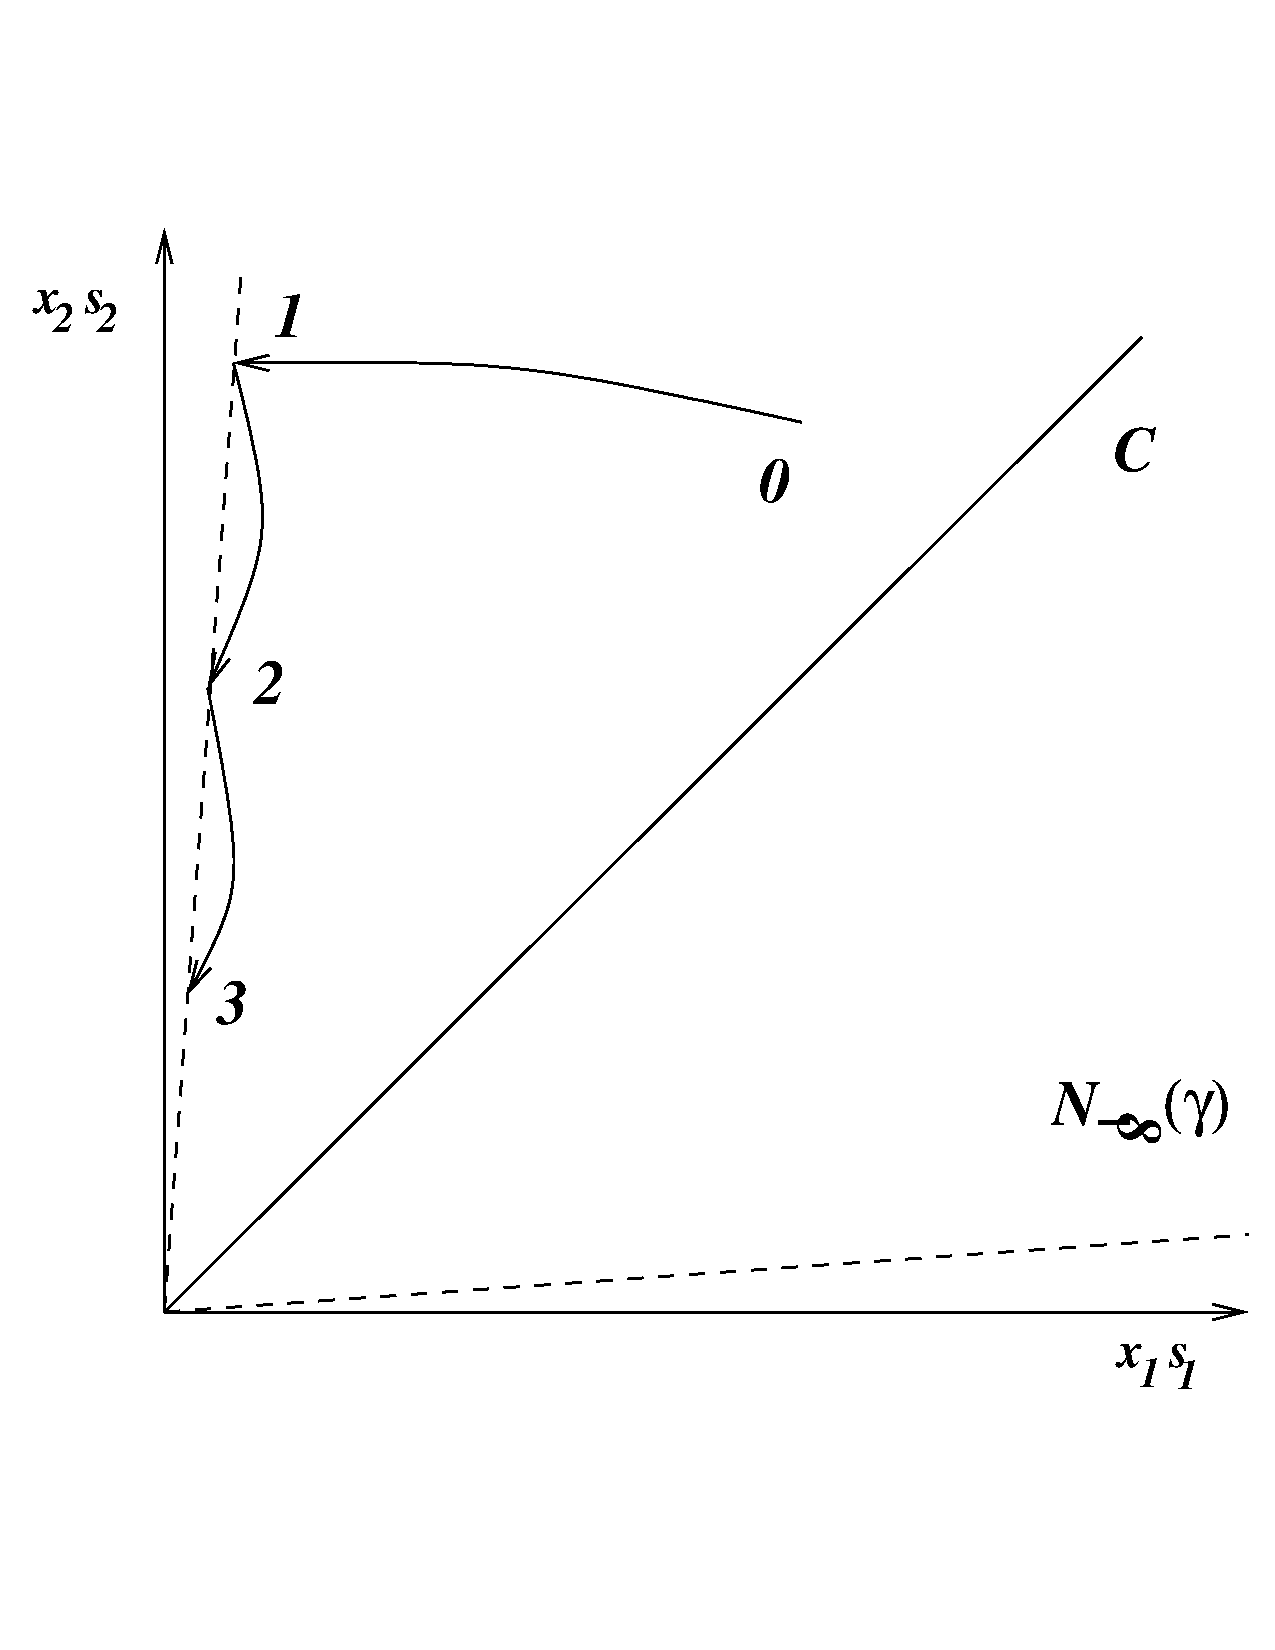
\includegraphics[width=3in]{figures/lecture26-central_path}
\end{center}
\caption{Require iterates to stay within a certain neighborhood of the central path.
We want the pairwise products $x_i s_i$ to be not too different for $i = 1, 2, . . . , n.$ }
\label{fig:figcentralpath}
\end{figure}

The goal is to find a tuple $(x, z, s)$ such that $\mu \approx 0$. We consider the following approach. Define
\begin{eqnarray*}
F_{\tau}(x,z,s) := \begin{bmatrix} Ax - b \\
A^\top z + s - c \\
x \circ s - \tau \mathbf{1} \\
\end{bmatrix}
\end{eqnarray*}
Then the goal is to approx solve $F_0(x_0,z_0,s_0) = \mathbf{0}$ over $\cF^0$. We see that this can be obtained by computing the solutions $(x_\tau,z_\tau,z_\tau)$ to $F_{\tau}(x,z,s) = \mathbf{0}$. We call the curve $\tau \mapsto (x_\tau,z_\tau,z_\tau)$ the ``central path''. Note that, on the central path, $x_i s_i = \tau$ for some $\tau > 0$. To ensure we stay close to the central path, we consider
\begin{eqnarray*}
\cN_{-\infty}(\gamma) &:=& \{(x,z,s) \in \cF_0: \min_i x_is_i \ge \gamma \mu(x,s)\}\\
\end{eqnarray*} 
What we would like to do is take iterates $(x_k,z_k,s_k)$ such that $\mu_k$ decreases, and $(x_k,z_k,s_k) \in  \cN_{-\infty}(\gamma)$ for appropriate constants $\gamma$. $\cN_{-\infty}(\gamma)$ ensures the nonnegativity contraints. This is portrayed in Figure \ref{fig:figcentralpath}.

\vspace{6mm}
\begin{algorithm}[h]
		\SetAlgoLined
		\textbf{Input:} Parameters $\gamma \in (0,1)$, $0 < \sigma_{\min} < \sigma_{\max} < 1$, and initialization $(x^0,z^0,t^0) \in \cN_{-\infty}(\gamma)$.
		\For{$t = 0,1,2,\dots$}{
		Choose $\sigma_{k} \in [\sigma_{\min},\sigma_{\max}]$\;
		Run Newton step on $F_{\sigma_k\mu_k}$ (to be defined). Let $(\Delta x^k, \Delta z^k, \Delta s^k)$ denote the Newton step
		\begin{eqnarray*}
		&&(\Delta x^k, \Delta z^k, \Delta s^k) = -\nabla^2 F_{\tau_k}(w^k)^{-1}\cdot \nabla F_{\tau_k}(w^k), \\
		&&\text{ where } \tau_k = \sigma_k \mu_k \text{ and } w^k = ( x^k, z^k, s^k)~.\;
		\end{eqnarray*}
		Let $\alpha_k \in (0,1]$ be the largest step such that
		\begin{eqnarray*}
		\alpha_k = \max \{\alpha \in (0,1]: (x^k,z^k, s^k) + \alpha (\Delta x^k, \Delta z^k, \Delta s^k) \in \cN_{\infty}(\gamma)\}	\;
		\end{eqnarray*}
		Set $(x^{k+1},z^{k+1}, s^{k+1}) \leftarrow (x^k,z^k, s^k) + \alpha_k (\Delta x^k, \Delta z^k, \Delta s^k)$.
		}
		\caption{Long-step Path Following method}\label{algLPF}
		\end{algorithm}

\subsection{Generating Iterates with the Newton Step}
	The Newton Step for solving fixed point equations $F(w) = 0$. Indeed
	\begin{eqnarray*}
	F(w+d) = F(w) + J(w)\cdot d + o(\|d\|)
	\end{eqnarray*}
	The Newton's method then chooses $w \leftarrow w + d$,
	\begin{eqnarray*}
	J(w)d = - F(w)
	\end{eqnarray*}
	Which implies that $F(w+d) = o(\|d\|)$ for $w$ sufficiently closed to the fixed point. This gives you the quick converge. Note that, if $F$ is a linear map, then in fact \emph{one Newton step suffices}. This can be seen from the Taylor expansion. 

\begin{figure}
\begin{center}
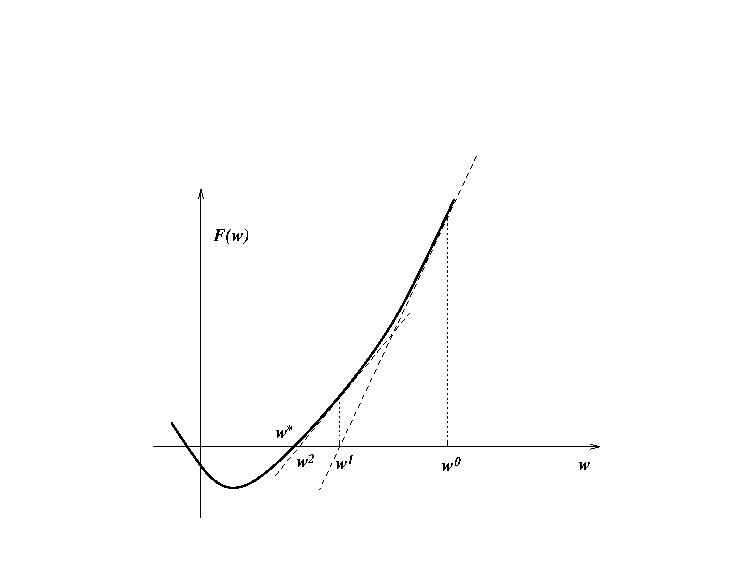
\includegraphics[width=3in]{figures/lecture26-newton}
\end{center}
\caption{ Recall that Newton's method iteratively finds better approximations to the roots (or zeroes) of a real-valued function.}
\end{figure}

	Our function $F_{\tau_k}$ is nearly linear, but not quite. Let's compute the Newton Step. We observe that the Jacobian is the linear operator
	\begin{eqnarray*}
	\begin{bmatrix}
	A & 0 & 0 \\
	0 & A^\top & I \\
	\mathrm{Diag}(S) & 0 & \mathrm{Diag}(X)
	\end{bmatrix}
	\end{eqnarray*}
	Moreover, since $(x^k,z^k,s^k) \in \cF^0$, we have that
	\begin{eqnarray*}
	F_{\tau_k}(x^k,z^k,s^k) = \begin{bmatrix} Ax^k - b \\
		A^\top z^k + s^k - c \\
		x^k \circ s^k - \tau_{k} \mathbf{1} \\
		\end{bmatrix} = \begin{bmatrix} 0 \\
		0 \\
		x^k \circ s^k - \tau_{k} \mathbf{1} \\
		\end{bmatrix}
	\end{eqnarray*}
	Let's drop subscripts. Then, on one can verify that the Newton satisfies
	\begin{eqnarray*}
	\begin{bmatrix}
	A & 0 & 0 \\
	0 & A^\top & I \\
	\mathrm{Diag}(S) & 0 & \mathrm{Diag}(X)
	\end{bmatrix} \begin{bmatrix} \Delta x\\
	\Delta z\\
	\Delta s
	\end{bmatrix} = \begin{bmatrix} 0 \\
	0 \\
	- x \circ s + \tau \mathbf{1} \\
	\end{bmatrix}
	\end{eqnarray*}

	Some remarks
	\begin{enumerate}
	\item $A \Delta x= 0$, and that $A^{\top} \Delta z + \Delta_s = 0$.
	\item This implies that $(x^+,z^+,s^+) := (x  + \Delta x, z+ \Delta z, s + \Delta s)$ satisfies
	\begin{eqnarray*}
	Ax^+ - b = 0\quad  \text{ and } \quad A^{\top} z^+ + s - c = 0\\
	\end{eqnarray*}
	\item We also have
	\begin{eqnarray*}
	s \circ \Delta x + x \circ \Delta s = - x \circ s + \tau \mathbf{1}
	\end{eqnarray*}
	and thus
	\begin{eqnarray*}
	x^+ \circ s^+ &=& x\circ s + \left( \circ \Delta x + x \circ \Delta s\right) + \Delta x \circ \Delta s\\
	 &=&  x \circ s - x \circ s + \tau \mathbf{1} + \Delta  x \circ \Delta s
	\end{eqnarray*}
	\item Thus, 
	\begin{eqnarray*}
	F_{\tau}(x^+\circ s^+) = \begin{bmatrix} 0 \\
	0 \\
	\Delta  x \circ \Delta s \\
	\end{bmatrix}
	\end{eqnarray*}
	In other words, if we can argue that $\Delta x \circ \Delta s$ is ``negligible'', then the Newton step produces an almost exact solution. 
	\end{enumerate}

	A more concrete analysis would be to study the term
	\begin{eqnarray*}
	n \mu(x + \alpha \Delta x, s + \alpha \Delta x)  &=& \langle x + \Delta x ,  s + \Delta s \rangle \\
	&=& \langle x , s \rangle  + \alpha \left(\langle x, \Delta s \rangle + \langle s, \Delta x \rangle \right) + \alpha^2 \langle \Delta s, \Delta x \rangle
	\end{eqnarray*}
	The last term in the above display vanishes, as shown by the above
	\begin{eqnarray*}
	0 = \Delta x^\top (A^{\top} \Delta z + \Delta s) = (A\Delta x)^\top z + \langle \Delta x, \Delta s \rangle = \langle \Delta x, \Delta \rangle
	\end{eqnarray*}
	Moreover, since $s \circ \Delta x + x \circ \Delta s = - x \circ s + \tau \mathbf{1}$, we have by summing that 
	\begin{eqnarray*}
	\langle x, \Delta s \rangle + \langle s, \Delta x \rangle =  - \langle x , x \rangle + \tau n = - (1 - \sigma) \langle x, s \rangle
	\end{eqnarray*}
	where the last line uses $n \tau = n \sigma \mu = \sigma n \tau =  \sigma \langle x, s \rangle$. Hence,
	\begin{eqnarray*}
	n \mu(x + \alpha \Delta x, s + \alpha \Delta x) = n \mu(x,s) (1 - \alpha(1-\sigma))
	\end{eqnarray*}
	Hence, if one can show that $(1-\alpha)\alpha \ge C(n) > 0$ for some constant depending on the dimension, then we see that
	\begin{eqnarray*}
	n \mu(x^{k+1}) \le (1 - C(n))^{k} n \mu(x^0)
	\end{eqnarray*}
	giving us the rate of decrease. One can then show with more technical work that $\alpha = \Omega(1/n)$ while maintaining the $\cN_{-\infty}(\gamma)$ invariant.
